\section{Introduction}

\IEEEPARstart{B}{iometrics} human characteristics and traits can successfully allow people identification and authentication and have been widely used for access control, surveillance, and also in national and global security systems~\cite{Jain:2008}.
In the last few years, due to the recent technological improvements for data acquisition, storage and processing, and also the scientific advances in computer vision, pattern recognition, and machine learning, several biometric modalities have been largely applied to person recognition, ranging from traditional fingerprint to face, to iris, and, more recently, to vein and blood flow. Simultaneously, various \emph{spoofing attacks} techniques have been created to defeat such biometric systems. 
% Therefore, the security of such systems against the myriad possible attacks is still an open problem~\cite{Pinto:SIBGRAPI:2012}.

There are several ways to spoof a biometric system~\cite{Rathgeb:ICPR:2010,Rathgeb:CVPRW:2011}. Indeed, previous studies show at least eight different points of attack~\cite{Galbally:DATABASE:2007,Ratha:AVBPA:2001} that can be divided into two main groups: \emph{direct} and \emph{indirect} attacks. The former considers the possibility to generate synthetic biometric samples, and is the first vulnerability point of a biometric security system acting at the sensor level. The latter includes all the remaining seven points of attacks and requires different levels of knowledge about the system, e.g., the matching algorithm used, the specific feature extraction procedure, database access for manipulation, and also possible weak links in the communication channels within the system.

%As an example, consider that an unauthorized user (an impostor) seeks to access a biometric-controlled system. If the user has some knowledge about the recognition system scores  (\emph{indirect attack}), the system can be easily circumvented and defeated~\cite{Adler:2008}.

Given that the most vulnerable part of a system is its acquisition sensor, attackers have mainly focused on direct spoofing. This is possibly because a number of biometric traits can be easily forged with the use of common apparatus and consumer electronics to imitate real biometric readings (e.g., stampers, printers, displays, audio recorders). 
In response to that, several biometric spoofing benchmarks have been recently proposed, allowing researchers to make steady progress in the conception of anti-spoofing systems. Three relevant modalities in which spoofing detection has been investigated are iris, face, and fingerprint. Benchmarks across these modalities usually share the common characteristic of being image- or video-based.

% This is precisely the focus of this work, i.e., to inves
%  (our focus herein)

% Although the definition of liveness detection (aka spoofing attack) is clear\footnote{Determining if the biometric being captured is an actual measurement from the authorized, live person who is present at the time of capture~\cite{Marcialis:ICIAP:2009}.}, most of the existing solutions in the literature address spoofing detection by presenting solutions custom-tailored for specific modalities.

In the context of irises, attacks are normally performed using printed iris images~\cite{Sequeira:IJCB:2014} or, more interestingly, cosmetic contact lenses~\cite{Bowyer:Computer:2014,Yadav:TIFS:2014}.
With faces, impostors can present to the acquisition sensor a photography, a digital video~\cite{Chingovska:BIOSEG:2012}, or even a 3D mask~\cite{Erdogmus:BTAS:2013} of a valid user. 
%
% (although much more expensive), it can use 
% In the latter case, the spoofing detection task is normally focused on the obfuscation of the iris texture due to the use of lenses rather than on the image telltales~\cite{Bowyer:Computer:2014,Yadav:TIFS:2014}.
%
For fingerprints, the most common spoofing method consists of using artificial replicas~\cite{Ghiani:ICB:2013} created in a cooperative way, where a mold of the fingerprint is acquired with the cooperation of a valid user and is used to replicate the user's fingerprint with different materials, including gelatin, latex, play-doh or silicone.
% Latent fingerprints left on a surface may also be used and further enhanced after acquisition with a digital camera. Then the negative fingerprint can be printed on a transparent sheet and used to attack a specific system.

The success of an anti-spoofing method is usually connected to the modality for which it was designed. In fact, such systems often rely on expert knowledge to engineer features that are able to capture acquisition telltales left by specific types of attacks. However, the need of custom-tailored solutions for the myriad possible attacks might be a limiting constraint. Small changes in the attack could require the redesign of the entire system.

In this paper, we do not focus on custom-tailored solutions. Instead, inspired by the recent success of Deep Learning in several vision tasks~\cite{Ciresan:2010,Krizhevsky:2012,Ciresan:2012,Ouyang:2014,Taigman:2014}, and by the ability of the technique to leverage data, we focus on two general-purpose approaches to build image-based anti-spoofing systems with convolutional networks for several attack types in three biometric modalities, namely iris, face, and fingerprint. The first technique that we explore is hyperparameter optimization of network architectures~\cite{Pinto:2009,Bergstra:2012} that we henceforth call \emph{architecture optimization}, while the second lies at the core of convolutional networks and consists of learning filter weights via the well-known back-propagation~\cite{LeCun:1998} algorithm, hereinafter referred to as \emph{filter optimization}.

 % to construct anti-spoofing systems from spoofing detection datasets

Fig.~\ref{f.schema} illustrates how such techniques are used. The architecture optimization (AO) approach is presented on the left and is highlighted in blue while the filter optimization (FO) approach is presented on the right and is highlighted in red. As we can see, AO is used to search for good architectures of convolutional networks in a given spoofing detection problem and uses convolutional filters whose weights are set at random in order to make the optimization practical. This approach assumes little a priori knowledge about the problem, and is an area of research in deep learning that has been successful in showing that the architecture of convolutional networks, by themselves, is of extreme importance to performance~\cite{Pinto:2009,Bergstra:2012,Saxe:2011,Pinto:2011b,Bergstra:2011,Bergstra:2013}. In fact, the only knowledge AO assumes about the problem is that it is approachable from a computer vision perspective.



\begin{figure}
\begin{center}
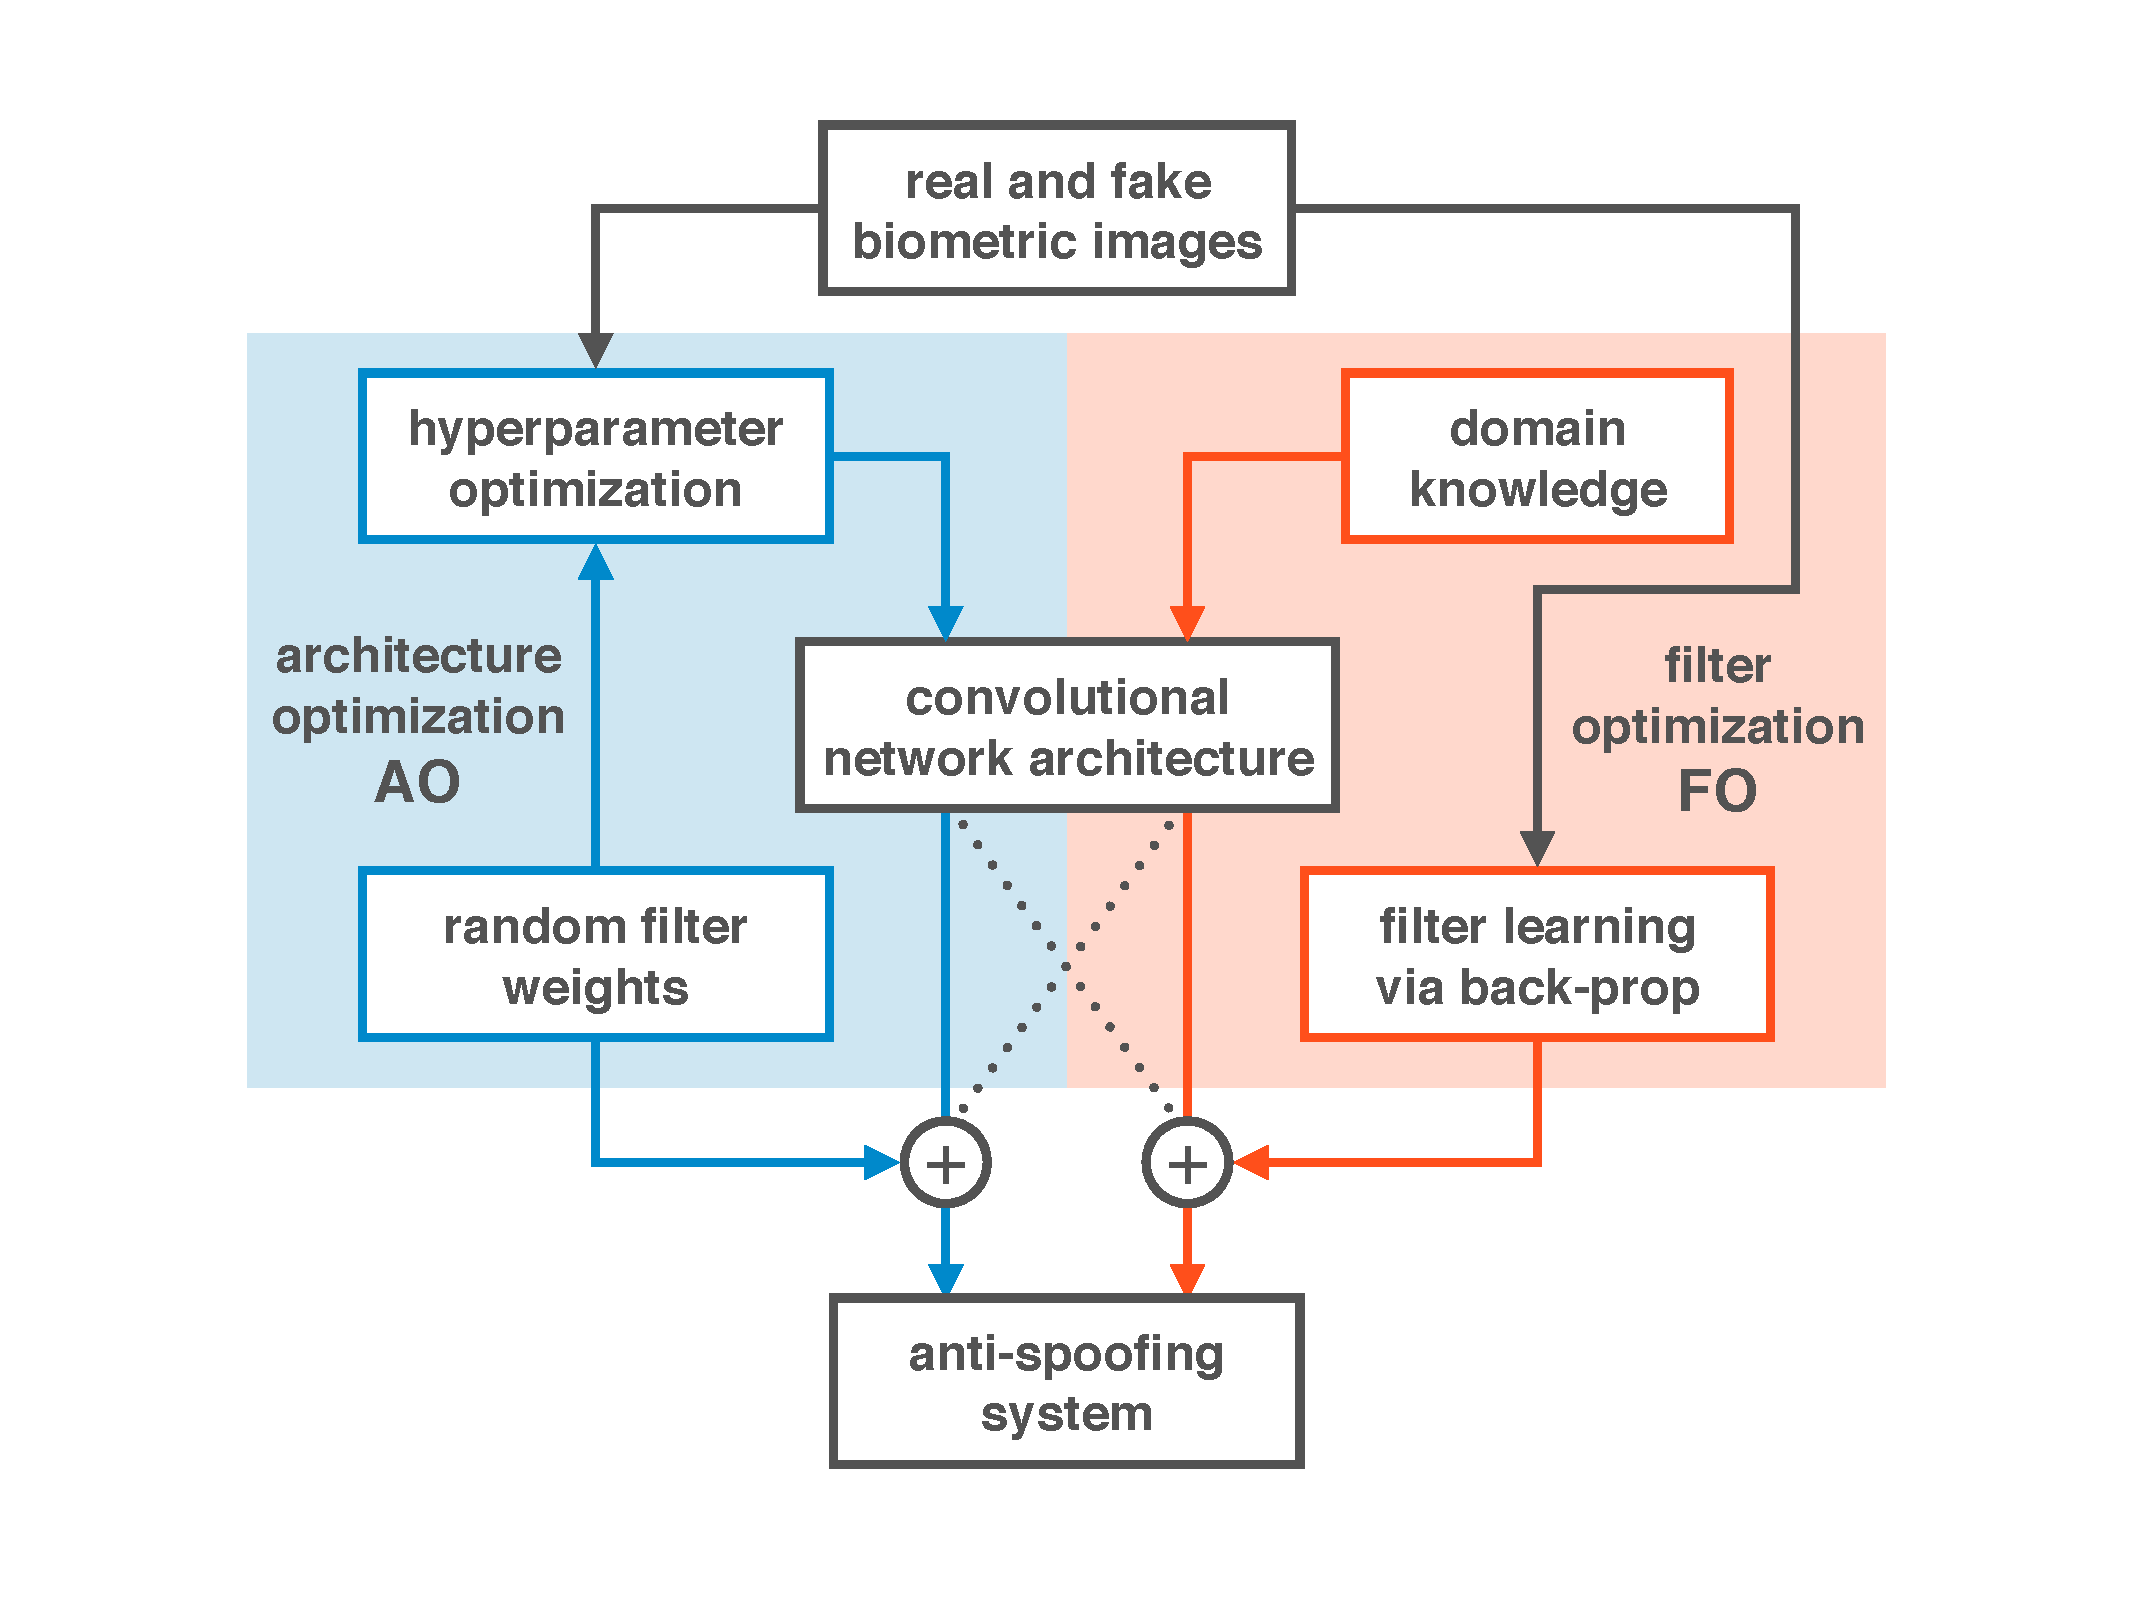
\includegraphics[width=0.9\linewidth]{schema.pdf} %% should be bring to 1.0\linewidth
\end{center}
\caption{Schematic diagram detailing how anti-spoofing systems are
  built from spoofing detection benchmarks. Architecture optimization
  (AO) is shown on the left and filter optimization (FO) on the
  right. In this work, we not only evaluate AO and FO in separate, but
  also in combination, as indicated by the crossing dotted lines.}
\label{f.schema}
\end{figure}

Still in Fig~\ref{f.schema}, FO is carried out with back-propagation in a predefined network architecture. This is a longstanding approach for building convolutional networks that has recently enabled significant strides in computer vision, specially because of an understanding of the learning process, and the availability of plenty of data and processing power~\cite{Krizhevsky:2012,Taigman:2014,Simonyan:2014}. Network architecture in this context is usually determined by previous knowledge of related problems.

% Both approaches, AO and FO, are used in this work to construct spoofing detection systems.

In general, we expect AO to adapt the architecture to the problem in hand and FO to model important stimuli for discriminating fake and real biometric samples. 
We evaluate AO and FO not only in separate, but also in combination, i.e., architectures learned with AO are used for FO as well as previously known good performing architectures are used with random filters.
This explains the crossing dotted lines in the design flow of Fig~\ref{f.schema}.

As our experiments show, the benefits of evaluating AO and FO apart and later combining them to build anti-spoofing systems are twofold.
First, it enables us to have a better comprehension of the interplay between these approaches, something that has been largely underexplored in the literature of convolutional networks. Second, it allows us to build systems with outstanding performance in all nine publicly available benchmarks considered in this work.

The first three of such benchmarks consist of spoofing attempts for iris recognition systems, Biosec~\cite{Ruiz-Albacete:BIOID:2008}, Warsaw~\cite{Czajka:MMAR:2013}, and MobBIOfake~\cite{Sequeira:VISAPP:2014:base}.
Replay-Attack~\cite{Chingovska:BIOSEG:2012} and 3DMAD~\cite{Erdogmus:BTAS:2013} are the benchmarks considered for faces, while Biometrika, CrossMatch, Italdata, and Swipe are the fingerprint benchmarks here considered, all them recently used in the 2013 Fingerprint Liveness Detection Competition (LivDet'13)~\cite{Ghiani:ICB:2013}. 


Results outperform state-of-the-art counterparts in eight of the nine cases and observe a balance in terms of performance between AO and FO, with one performing better than the other depending on the sample size and problem difficulty. In some cases, we also show that when both approaches are combined, we can obtain performance levels that neither one can obtain by itself. Moreover, by observing the behaviour of AO and FO, we take advantage of domain knowledge to propose a single new convolutional architecture that push performance in five problems even further, sometimes by a large margin, as in CrossMatch (68.80\% \emph{v.} 98.23\%).  

The experimental results strongly indicate that convolutional networks can be readily used for robust spoofing detection.  
Indeed, we believe that data-driven solutions based on deep representations might be a valuable direction to this field of research, allowing the construction of systems with little effort even to image-based attack types yet to come.

% in which we propose the use of a general pipeline for spoofing detection able to automatically learn representative and discriminative features from the available training data without the need for expert custom-tailored solutions. 

% \rva{We explore two deep learning research branches of the literature and discuss their pros and cons, optimizing architectures \emph{vs.} learning filter weights (via back-propagation). Finally, we also extend existing approaches in the literature showing that the knowledge of the domain still plays an important role and can also improve deep-learning based solutions. We explore two approaches in deep representation learning to derive outstanding spoofing detection systems for iris~\cite{LivDet:Iris:2013,Sequeira:IJCB:2014}, 
% face~\cite{Chakka:IJCB:2011,Chingovska:ICB:2013}, and fingerprint~\cite{Marcialis:ICIAP:2009,Yambay:ICB:2012,Ghiani:ICB:2013} biometric modalities.}

%\rva{The deep representations~\cite{Bengio:2013} we consider are biologically inspired and have been successfully used in the face recognition context~\cite{Pinto:2011,Chiachia:2012,Chiachia:2014} by our team. It also has been recently employed by our team for handheld printed iris spoofing attacks with promising results~\cite{Sequeira:IJCB:2014}.}

%We consider nine biometric spoofing benchmarks — each one containing real and fake samples of a given biometric modality and attack type — and learn systems for each benchmark by combining and contrasting the two learning approaches.

% Deep learning (DL) techniques have shown a great success in several computer vision tasks with groundbreaking results~\cite{Ciresan:2010,Krizhevsky:2012,Ciresan:2012,Ouyang:2014,Taigman:2014} for many difficult problems. 
% Allied with their success, DL techniques enable us to learn multi-layered (hence the term deep) representations directly from the data. 
% This powerful representation allows us to find deep representational connections that would be hardly thought by a human expert.

% The learned representations model the distribution of real and fake classes yielding outstanding liveness detection methods~\cite{Sequeira:IJCB:2014}.
% Here, we are particularly interested in the use of a specific type of technique for learn deep representations: the convolutional neural networks (CNN), which was initially introduced by LeCun \emph{et al.}~\cite{LeCun:1998}.

% By exploring the two most important research paths (architecture optimisation \emph{vs.} filter weight learning) in deep learning representation, we are able to study their impacts, pros and cons when adapted for the spoofing attack detection problem. The first approach consists of searching for suitable architectures of convolutional networks operating in problem domains, whilst the second approach focuses on learning filter weights via back-propagation seeking to model important stimuli for discriminating fake and real biometric samples. 

% \rva{Optimizing the network architecture and its hyper-parameter space has been explored successfully in vision problems by~\cite{}. Complementing, learning the network weights of a CNN with a predefined topology was explored by~\cite{Jarrett:2009,Krizhevsky:2012,Taigman:2014} while~\cite{Coates:2011,Le.Quoc:2012,Coates:2013} estimated the weights using an unsupervised learning algorithm. On the top of these learned representations either optimising the architecture or learning filter weights or both, we attach a discriminative classifier, the Support Vector Machines (SVMs) with linear kernels and hard margins~\cite{Cortes_Vapnik:1995,Chang:2011}. Other classifiers could be considered here as well. In the architecture optimization, we study and analyze the use of random search techniques~\cite{Pinto:2009,Pinto:2011b,Bergstra:2012,Bergstra:2011,Bergstra:2013}.}

% \rva{In this work, we consider nine publicly available benchmarks: three of iris printed spoofing attacks (Biosec~\cite{Ruiz-Albacete:BIOID:2008}, Warsaw~\cite{Czajka:MMAR:2013}, and MobBIOfake~\cite{Sequeira:VISAPP:2014:base}), two of face (Replay-Attack~\cite{Chingovska:BIOSEG:2012} and 3DMAD~\cite{Erdogmus:BTAS:2013}) and four of fingerprint spoofing attacks used in the latest, 2013, Fingerprint Liveness Detection Competition (LivDet'13)~\cite{Ghiani:ICB:2013} (Biometrika, CrossMatch, Italdata, and Swipe). The obtained results outperform the best known results for faces, fingerprints, and iris spoofing detection in eight out of the nine considered benchmarks, 
% sometimes reducing their classification error in more than 30 percentage points (e..g, for the CrossMatch spoofing fingerprint benchmark, 98.23\% \emph{v.} 68.80\%).}

% It is worth mentioning that, recently, Galbally et al.~\cite{Galbally:TIP:2014}  was one of the first authors to propose a unified countermeasure method to detect spoofing attacks in face, iris, and fingerprint biometric systems. Their solution is based on image quality assessment. According to the authors, a spoofing attack can be detected by using 25 general image quality features extracted from one image. 
% The experimental results reported attest the effectiveness of the method and its high competitiveness compared to other approaches. We see this work as the most related to ours, therefore, it is also worth mentioning a few key differences between these solutions. 
% \rva{First and foremost, our method does not rely on image quality features, rather it automatically learns representational and discriminative features directly from the data using a deep learning framework. Second, our solution has been evaluated in more recent and updated databases which makes the comparison not straightforward. However, regardless of the differences, we believe that solutions able to automatically learn representations directly from the data for spoofing detection should be the path taken for future researchers in the field.}


We organized the remainder of this work into five sections.
Section~\ref{sec:relatedwork} presents previous anti-spoofing systems for the three biometric modalities covered in this paper, while Section~\ref{sec:databases} presents the considered benchmarks. Section~\ref{sec:methodology} describes the methodology adopted for architecture optimization (AO) and filter optimization (FO) while Section~\ref{sec:experiments} presents experiments, results, and comparisons with state-of-the-art methods. Finally, Section~\ref{sec:conclusions} concludes the paper and discusses some possible future directions.
